\documentclass[a4paper]{article}
\usepackage[utf8]{inputenc}
%Pacote de linguagem
\usepackage[utf8]{inputenc}

%Regras da ABNT
\usepackage[lmargin=3cm, rmargin=2cm, tmargin=3cm, bmargin=2cm]{geometry}
\usepackage[onehalfspacing]{setspace}
\usepackage[brazil]{babel}

%Importando pacote de fontes
\usepackage[T1]{fontenc}
\usepackage{mathptmx}


%Importando bibliotecas essenciais
\usepackage{graphicx, xcolor, comment, indentfirst, enumerate, multirow, multicol, color, hyperref, float}

%Importante bibliotecas matemáticas
\usepackage{amsmath, amsthm, amsfonts, amssymb, dsfont, mathtools}

%Comandos novos

\newcommand{\HRule}{\rule{\linewidth}{0.5mm}}

\begin{document}


% ----------------------- CAPA --------------------------

\begin{titlepage}
% Imagem
\centering 
\includegraphics[width=0.4\linewidth]{images/fametro.png}

%Faculdade e materia
\textsc{\textbf{\Large Faculdade Metropolitana de Manaus - FAMETRO}}\\[0.5cm]
\textsc{\textbf{\Large Gestão de Processo de Negócios}}\\[0.5cm]

%Titulo
\vspace{1.0cm}
\HRule \\[0.4cm]
{\huge \textbf{DESIGN THINKING}} \\[0.25cm]
\HRule \\[1.0cm]
\vspace{1.0cm}

%Professora
\textbf{\Large Profª: Zaida Tavares} \\[0.4cm]
\vspace{0.5cm}
%Alunos
\begin{flushright}
    \begin{tabular}{r|l}
            Joelson Lima & RM: 2142448 \\
            Natanael Falcão & RM: 2015893 \\
            Jessé Freitas & RM: 2019384 \\
            Augusto Alejandro & RM: 2018230 \\
            America Tereza & RM: 2022949 \\
            David Teixeira & RM: 2021469
    \end{tabular}
\end{flushright}

\vfill
%Informações de local e data
\textbf{\large Manaus - AM}\\[0.5cm]
\textbf{\large 2021}

\end{titlepage}

% ----------------------- SUMÁRIO --------------------------
\section{Sumário}

%Itens do sumário
\begin{itemize}
    \item[2.] Introdução \dotfill 2
    \item[3.1.] Empatia Funcionários \dotfill 3
    \item[3.2.] Empatia Usuários \dotfill 4
    \item[3.3.] Imersão \dotfill 5
    \item[3.4.] Análise e Síntese \dotfill 6
    \item[3.5.] Ideação ou Ideation \dotfill 6
    \item[3.6.] Prototipação ou Prototipagem \dotfill 7
    \item[3.7.] Resultado das Entrevistas \dotfill 7
    \item[4.] Conclusão \dotfill 9
    \item[5.] Bibliografia \dotfill 10
\end{itemize}
\vfill
\pagebreak
% ----------------------- INTRODUÇÃO --------------------------
\section{Introdução}
\par O Design Thinking é uma metodologia utilizada para oferecer produtos e serviços de acordo com a real necessidade dos clientes. Ela é cada vez mais utilizada por empresas que desejam aperfeiçoar seus serviços de forma simples, ágil e bem planejada, uma vez que ela aproveita características de um profissional de designer — como sua forma de pensamento, potencial criativo e empatia — em todo o negócio e não apenas na criação de um só produto.
\par O Design Thinking vai além da estética de produtos ou serviços. No mundo dos negócios, está relacionado com inovação.
\subsection{Empresa: Google}
\par Uma das maiores empresas de tecnologia do mundo, o Google completou 20 anos de existência. A companhia foi fundada por Larry Page e Sergey Brin, que se conheceram na universidade de Stanford, na Califórnia, e se uniram para desenvolver um novo motor de buscas. Em 1998, o primeiro escritório do Google foi montado dentro da garagem Susan Wojcicki – que mais tarde se tornaria CEO do YouTube. Desde então, a empresa expandiu sua atuação para múltiplos setores, ajudando a revolucionar a forma como lidamos com a tecnologia atualmente. \\[1cm]
\begin{figure}[h]
    \centering
    
\includegraphics[width=4cm]{images/google_logo.png}
    \caption{Logo da Google}
    \label{fig:my_label}
\end{figure}




\vfill
\pagebreak


% ----------------------- DESENVOLVIMENTO --------------------------
\section{Desenvolvimento}
\subsection{Empatia Funcionários}
\begin{figure}[h]
    \centering
    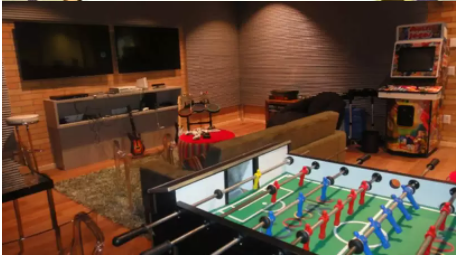
\includegraphics[width=7cm]{images/empatia_func.png}
    \caption{Conforto no local de trabalho}
\end{figure}

\par Estratégia de trazer um ambiente de trabalho moderno e descontraído, muito se fala sobre os escritórios do Google em todo mundo, por serem conhecidos por ambientes modernos e descolados. Mas os segredos do Google para motivar e gerar engajamento entre seus funcionários vão além disso.
\par Após extensa pesquisa com funcionários, a empresa de tecnologia entendeu que as formas como os membros da equipe interagem, estruturam seu trabalho e enxergam sua contribuição são mais importantes até mesmo do que quem faz parte da equipe.
\par Para o próprio Google, o segredo da motivação e engajamento de seus funcionários está fundamentado em uma lista de aspectos. Confira quais são eles: 

\begin{itemize}
    \item Segurança Psicológiga
    \par Quem trabalha no Google pode se sentir seguro para arriscar e questionar sem medo de ser repreendido. Essa segurança estimula os funcionários a dar ideias e ser colaborativos.  “A cultura do Google incentiva a fazer perguntas e compartilhar informações. Para replicar seu sucesso, crie um ambiente de equipe que convide e extraia contribuições de todos os membros”, acredita Robert Bruce Shaw.
    
    \item Confiabilidade
    \par Trabalho colaborativo na prática é outro ponto importante. Colaboradores do Google podem contar uns com os outros, e isso tem ajudado a melhorar o ambiente de trabalho. Uma das iniciativas neste sentido é o Googler-to-Googler (G2G), programa no qual mais de seis mil funcionários se oferecem para ajudar seus colegas. 
    \par Outro aspecto relevante é destacado por Lucy Ford, professora de administração da Saint Joseph’s University’s Haub School of Business. Segundo ela, os funcionários do Google podem usar 20\% de sua carga horária de trabalho para desenvolver suas próprias ideias inovadoras. “O que é crítico é que os funcionários não são obrigados a gastar 20\% do seu tempo em seus próprios projetos, mas, se eles escolherem, isso é incentivado”, afirmou a Fast Company.

    \item Estrutura e Clareza
    \par Uma preocupação da empresa é que metas, funções e planos de execuções estejam claros para as equipes.  A empresa também cita a transparência como um fator importante. Permitir, por exemplo, que os funcionários acessem códigos base e outras informações internas. “Acreditamos que, se você tiver boas pessoas e acreditar que elas são fundamentalmente boas, elas tomarão melhores decisões se forem expostas ao que está acontecendo na organização”, já declarou Laszlo Bock, ex-vice-presidente sênior de operações com pessoas do Google.
    
    \item Significado e Impacto do Trabalho
    \par A empresa sabe que o emprego tem importância para seus colaboradores e que eles acreditam que seus trabalhos podem gerar mudanças. Esse entendimento por parte da empresa cria empatia com suas equipes, em vez de divisões hierárquicas. “As pessoas querem trabalhar em algo significativo, que faça a diferença para sua organização e para a sociedade em geral”, afirmou Shaw na entrevista para a Fast Company.
\end{itemize}
\subsection{Empatia Usuários}
\begin{figure}[h]
    \centering
    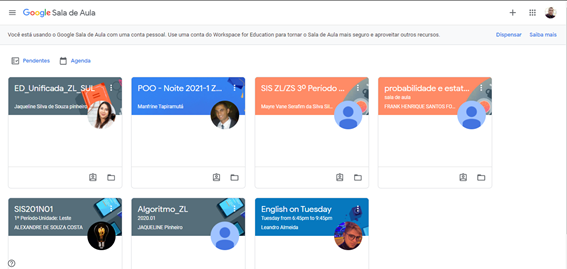
\includegraphics[width=15cm]{images/empatia_user.png}
    \caption{Facilidade de acesso para o usuário}
\end{figure}
\par São evidentes as transformações no modo de vida das pessoas ao redor do mundo, no momento pelo qual passamos. Dentre estas adaptações está o aumento do uso das Tecnologias de Comunicação e dos dispositivos eletrônicos, como celulares e computadores, em conexão com a Internet e, mais especificamente, o uso do Google. Empresas que oferecem serviços de e-mail, e-comerce (lojas virtuais), EAD, e muitos outros, ganharam espaço na web em decorrência da crescente procura.
\par Nessa perspectiva, percebemos claramente a presença do Google, na maioria dos processos online. Até quando, sequer percebemos, nas páginas que acessamos, ele está lá, presente em em algum processo, ou através de alguma de suas ferramentas.\\
\begin{center}
    \textbf{\large “Apenas uma conta. Tudo o que o Google oferece”.}\\[0.8cm]
\end{center}
\par Com esta frase, somos convidados a abrir uma conta na página inicial do Google, antes de aceitarmos (muitas vezes, sem uma leitura cuidadosa) os termos de compromisso. Podemos interpretar o slogan como: “numa conta, você tem todos os serviços e possibilidades que o Google te oferece”. 
\par Os impactos do Google atingem também a educação, vale ressaltar que os resultados de pesquisas são dispostos não só com base na relevância, mas também nos ‘hábitos de busca’ dos usuários, essa contribuição vem ajudando estudantes e instituições de ensino.\\[1.5cm]
\subsection{Imersão}
\begin{figure}[h]
    \centering
    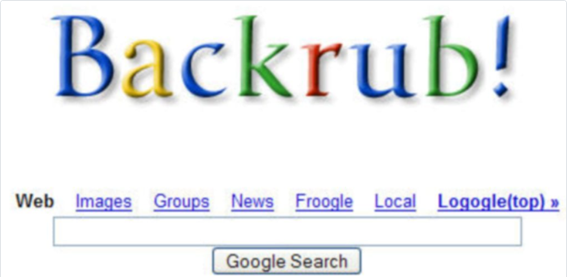
\includegraphics[width=10cm]{images/imersão.png}
    \caption{Backrub!, nome original do Google}
\end{figure}
\par Com o surgimento da internet em passos largos, foram surgindo pequenos negócios em garagens e faculdades, o mesmo foi com os criadores do Google, Larry Page e Sergey Brin.
Além disso, os dois se tornaram parceiros de pesquisa, estudando as propriedades matemáticas da internet. Com a dissertação “The Anatomy of a Large-Scale Hypertextual Web Search Engine” (A anatomia de um mecanismo de pesquisa da Web hipertextual em grande escala, em tradução livre), descreviam especificidades de um buscador capaz de rastrear a web e ranquear as páginas por relevância. Dessa maneira, decidiram criar a página que se tornaria o Google.\\[0.3cm]

\par \textbf{\large Fatores Internos Positivos}
\begin{itemize}
    \item "Almas gêmeas intelectuais"
    \item Conhecimento Informática
    \item A proximidade com pessoas
    \item Ambiente de trabalho
\end{itemize}

\par \textbf{\large Fatores Internos Negativos}
\begin{itemize}
    \item Falta de capital de investimento
    \item Toma todo seu tempo
    \item Honestidade entre colegas
\end{itemize}  

\par \textbf{\large Fatores Externos Positivos}
\begin{itemize}
    \item Um e-mail, vários serviços
    \item Melhor ferramenta de busca
    \item Armazenamento grátis
\end{itemize}

\par \textbf{\large Fatores Externos Negativos}
\begin{itemize}
    \item Acesso aos dados das pessoas
    \item Manipulação de produtos
    \item Exclusão de usuários
\end{itemize}

\subsection{Análise e Sintese} 
\begin{figure}[H]
    \centering
    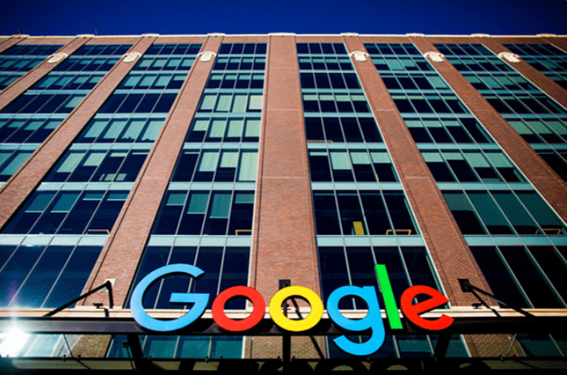
\includegraphics[width=10cm]{images/analise.png}\\[0.5cm]
    \caption{Google atualmente}
\end{figure}
\par O Google é uma empresa multinacional de serviços online e software dos Estados Unidos. Principal subsidiária da Alphabet, ela hospeda e desenvolve uma série de serviços e produtos baseados na internet e gera lucro, principalmente, por meio da publicidade pelo AdWords.
\par O rápido crescimento do Google desde sua incorporação culminou em uma cadeia de outros produtos, aquisições e parcerias que vão além do núcleo inicial como motor de buscas. A empresa oferece softwares de produtividade online, como o software de e-mail Gmail, e ferramentas de redes sociais, incluindo o Google+.
\par Com todo esse crescimento a empresa ainda precisa de mais flexibilidade em relação a liberdade de seus usuários, muitas denúncias de violação de privacidade e também de exclusão de seus serviços por razões desconhecidas e até mesmo ideológica.

\subsection{Ideação ou Ideation}
\begin{figure}[h]
    \centering
    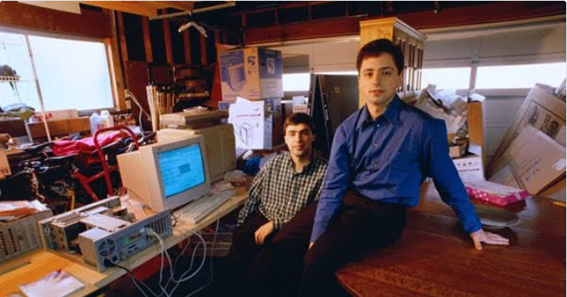
\includegraphics[width=10cm]{images/ideacao.png}\\[0.5cm]
    \caption{Criadores do Google}
\end{figure}
\par Os dois buscaram financiamento para conseguir abrir a companhia e chegaram até mesmo a se endividar com amigos. Durante essa fase, Page e Brin conseguiram um bom crescimento e tentaram vender sua startup. A dupla ofereceu o site de buscas ao portal Excite por US\$ 1 milhão, mas não teve sucesso.

\subsection{Prototipação ou Prototipagem}
\begin{figure}[h]
    \centering
    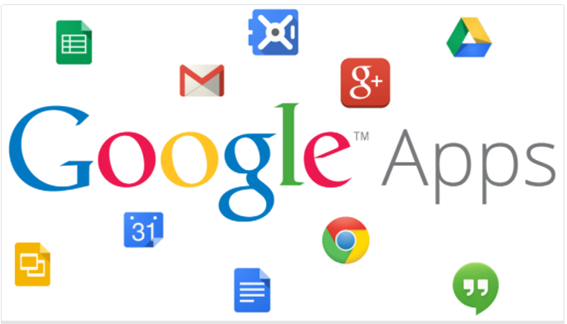
\includegraphics[width=10cm]{images/proto.png}\\[0.5cm]
    \caption{Vários apps criados pela Google}
\end{figure}
\par Com o sistema já desenvolvido a partir de um trabalho desenvolvido na faculdade, o Google entrou em funcionamento em janeiro de 1996, a partir daí a dupla começou a focar na evolução da empresa.
\par O crescimento da empresa nos anos 2000 começa a dar forma a história do Google. Em maio, o site passou a ter versões em idiomas além do inglês, incluindo o português. As outras línguas adicionadas foram: francês, alemão, italiano, sueco, finlandês, espanhol, holandês, norueguês e dinamarquês.
\par O sucesso foi tanto que o buscador do Yahoo! passou a utilizar o serviço do Google em seu portal. No mesmo ano, o site chegou a um bilhão de endereços categorizados e ampliou o serviço para japonês, chinês e coreano. Entretanto, a China começou com bloqueios ao sistema. Eventualmente, o bloqueio a qualquer conteúdo internacional foi decretado.
\par A partir do fim do ano, o Google passou a investir em serviços além da busca. Foi nessa época que a empresa comprou o Usenet Discussion Service. O serviço foi renomeado para Google Groups e oferecia um espaço para discussões online.

\subsection{Resultados das Entrevistas}
\par As pesquisas foram feitas de forma virtual. \href{https://docs.google.com/forms/d/1R7aUG0Rk3e8IBl5C9skZ4EZBTYdEt05p6FwKriKgc9E/edit#responses}{\color{blue}Clique aqui para ver os resultados}\\
\begin{center}
    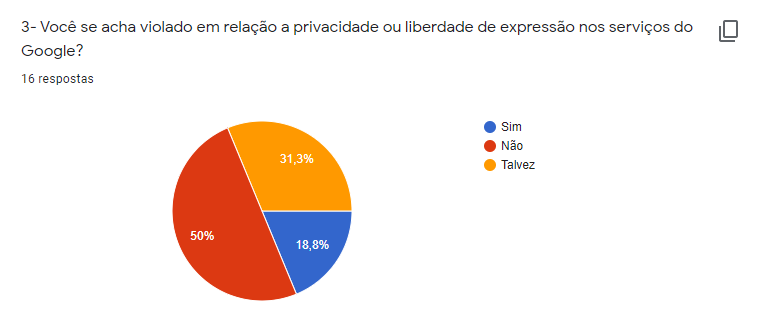
\includegraphics[width=0.8\linewidth, height=6cm]{images/graph_1.png}\\[1cm]
    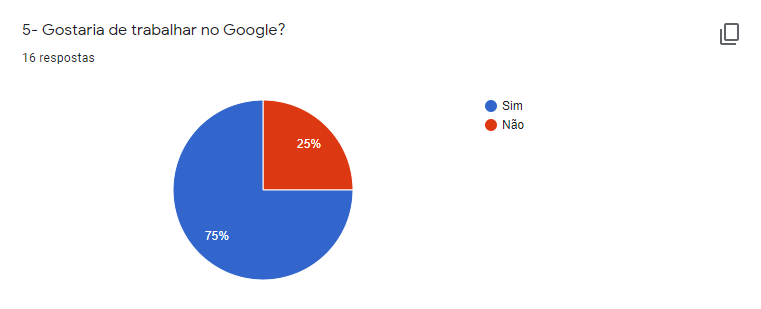
\includegraphics[width=0.8\linewidth, height=6cm]{images/graph_2.png}
\end{center}
\par \textbf{Qual é a sua visão da empresa Google, em relação aos usuários? Ex. Benefícios e malefícios.}
\par \textit{“É uma ótima empresa, me ajuda em diversas pesquisas e em tradução de diversos textos nos mais variados idiomas. No momento eu não consigo achar nenhuns malefícios.”} - \textsc{Gabriel Ribeiro – Químico} \vspace{1mm}
\par \textbf{Você se acha violado em relação a privacidade ou liberdade de expressão nos serviços do Google?}
\par \textit{“Sim”} - \textsc{Silas Castro - Desenvolvedor Web} \vspace{1mm}
\par \textbf{Qual é a sua visão da empresa Google, em relação aos usuários? Ex. Benefícios e malefícios.}
\par \textit{“Benefícios é que existem muito serviços de boa qualidade na conta do Google e malefício que te torna muito depende somente das plataformas do Google.”
} - \textsc{David - Tecnólogo da informação} \vspace{1mm}
\par \textbf{Quais serviços do Google você mais gostou ou gosta?}
\par \textit{“Google Docs e Spreadsheets pra organizar dados e trabalhar mais eficientemente com compartilhamento de documentos em equipe”} - \textsc{Joelson Lima - Estudante} \vspace{1mm}
\par \textbf{Se você estivesse no controle, o que você faria para melhorar a empresa Google?}
\par \textit{“Pararia de roubar e vender os dados dos usuários, cansei de propaganda safada”} - \\ \textsc{José Elias – Estudante}


\vfill
\pagebreak
% ----------------------- CONCLUSÃO --------------------------
\section{Conclusão}
\par A empresa Google começou a partir de uma necessidade, mas precisou aplicar técnicas de gerenciamento para amadurecer, ter empatia com seus funcionários e usuários foi e é muito importante para o Google chagar ao sucesso e permanecer, mesmo com sucesso também existem muitas mudanças a serem realizadas para se adequar as exigências de seus usuários.
\par Adotar o Design Thinking como abordagem em sua empresa é uma ação que pode fazer a diferença no futuro do seu negócio. A partir dele é possível encontrar soluções criativas, eficientes e baratas para diversos problemas, desde assuntos internos até o lançamento de novos produtos e serviços.


\vfill
\pagebreak
% ----------------------- BIBLIOGRAFIA --------------------------
\section{Bibliografia}
\begin{itemize}
    \item SILVA, Maurício José Vianna e; FILHO Ysmar Vianna e Silva; ADLER, Isabel Krumholz; LUCENA, Brenda de Figueiredo; RUSSO, Beatriz - \textbf{Design Thinking - Inovação em Negócios}. 2ª Ed. eletrônica. RIO DE JANEIRO, RJ: MJV Techlonogy \& Innovation, 2018.
    
    \item O que é Design Thinking: conceitos e definições, Meu Sucesso, 2014. Disponível em: \textbf{\\ https://meusucesso.com/artigos/inovacao-e-tecnologia/o-que-e-design-thinking-conceitos-e-definicoes-\\132/}.
    \\Acesso em 11 de setembro de 2021.
    
    \item Como o Google motiva seus funcionários, SA Varejo, 2018. Disponível em: \textbf{\\https://www.savarejo.com.br/detalhe/reportagens/como-o-google-motiva-seus-funcionarios}.
    \\Acesso em 11 de setembro de 2021.
    
    \item 20 momentos e produtos que marcaram a história do Google, The Enemy, 2018. Disponivel em: \textbf{\\https://www.theenemy.com.br/tech/20-momentos-e-produtos-que-marcaram-a-historia-do-google}. \\Acesso em 11 de setembro de 2021.
    
    \item A história do Google, Oficina da Net, 2019. Disponivel em:  \textbf{\\https://www.oficinadanet.com.br/post/14208-a-historia-do-google}.
    \\Acesso em 11 de setembro de 2021.
\end{itemize}
\end{document}
